\chapter{Proposta de Solução}
\label{cap:proposta}

A solução proposta para permitir a realização de experimentos de plataformas de Cidades Inteligentes em ambientes simulados abrangendo diferentes cenários em diferentes escalas será
apresentada neste capítulo.
A discussão sobre os requisitos de uma possível solução para esse problema será feita, levando em consideração as principais dificuldades para a criação de um ambiente como esse.
Além disso, uma arquitetura de software para uma solução será apresentada, sabendo que uma arquitetura de software para um sistema é a estrutura ou estruturas do sistema, que compreende elementos,
seu comportamento externamente visível e as relações entre eles~\cite{clements_2002}.

\section{Requisitos da Solução}
\label{sec:requisitos}

Para a realização de experimentos em ambientes simulados de Cidades Inteligentes temos requisitos em diferentes níveis, desde a capacidade do simulador de representar o contexto
de uma cidade até formas de comunicação que permita a interação entre o simulador e a plataforma de Cidades Inteligentes.
Portanto, dividimos os requisitos em \textbf{fundamentais} e de \textbf{integração}.

Para que o simulador possa refletir o contexto de Cidades Inteligentes, onde o sensoriamento de diversos aspectos das cidades já é uma realidade, e a atuação (modificação do estado
das cidades) segue uma crescente, consideramos que a mesma deva ter de alguma forma representada os conceitos abaixo:

\begin{itemize}
    \item \textit{Modelos aderentes a realidade de uma cidade}: o simulador deve implementar modelos que representem ao máximo a realidade de uma cidade, e não apenas casos hipotéticos.
        Por exemplo, modelos de fluxo de automóveis nas vias devem incluir possíveis engarrafamentos.

    \item \textit{Execução com noção de tempo real}: a dinâmica da cidade deve ser simulada em tempo real, ou seja, não deve ser executada nem mais rápida nem mais lenta do que aconteceria
        em um ambiente real de uma cidade (um segundo simulado é aproximadamente igual a um segundo real).
        Esse é um requisito importante, pois o desencadeamento de ações nas cidades são muitas vezes devido ao processamento de ações acontecidas anteriormente, e as plataformas
        devem ter tempo hábil para realizar tais ações, como foi explicado nos capítulos anteriores.

    \item \textit{Geração de grande massa de dados}: para realizarmos experimentos realistas devemos ser capazes de gerar uma massa de dados na mesma escala de uma grande cidade por
        exemplo.
        Experimentos em escalas menores são úteis na validação de certos cenários, contudo não exercita uma plataforma de Cidades Inteligentes em um contexto real, onde deverá
        interagir com milhões de sensores, atuadores e usuários.

    \item \textit{Comunicação em tempo de execução}: para que esse ambiente integrado seja viável, ambas as ferramentas devem ser capazes de se comunicarem em tempo de execução.
        Com isso, se torna possível a envio de dados de sensores e comandos de atuação durante a emulação.
\end{itemize}

Consideramos os pontos apresentados acima como \textbf{requisitos fundamentais}, sendo esses o mínimo necessário para conseguirmos de fato representar um ambiente real de uma cidade.
Caso a ferramenta atenda os requisitos apresentados, se torna possível a simulação de cenários realistas no contexto de Cidades Inteligentes, podendo substituir \textit{testbeds}
reais, em uma escala maior, após a sua integração com a plataforma alvo.
Todavia, apenas essa simulação não viabiliza ainda a realização de experimentos com plataformas, ainda precisamos atender alguns \textbf{requisitos de integração} entre o simulador
e a plataforma em questão.

Para termos um ambiente integrado precisamos definir um meio de comunicação de duas vias, envio e recebimento de dados, em tempo real entre o simulador e a plataforma de Cidades Inteligentes.
Além disso, deve haver uma integração semântica que viabilize as ferramentas se comunicarem de maneira eficaz.
Abaixo são apresentados os \textbf{requisitos de integração} necessários para obtermos um ambiente integrado de experimentação para essas plataformas:

\begin{itemize}
    \item \textit{Integração semântica}: para que seja possível a comunicação em tempo de execução entre o simulador e a plataforma, ambos precisam entrar em um consenso semântico.
        Abaixo são apresentados os dois principais conceitos envolvidos e que acreditamos que seja necessário serem representados de alguma forma em ambas as ferramentas para que seja
        possível a integração.

        \begin{itemize}
            \item \textit{Recursos da cidade}: esse recursos da cidade, sendo eles qualquer coisa no contexto da cidade (automóveis, aparelhos públicos, vias e etc.), serão objetos tanto de
                sensoriamento e/ou atuação por parte das plataformas de Cidades Inteligentes.

            \item \textit{Capacidades inerentes a cada recurso da cidade}: cada \textit{recurso da cidade} tem as suas respectivas capacidades, sendo elas de sensoriamento ou atuação.
                Essas capacidades usualmente estão atreladas a dispositivos heterogêneos de IoT (\textit{Internet Of Things}) presentes nos recursos da cidade.
                Por exemplo, vagas de estacionamento podem ser monitoradas quanto a sua ocupação, e semáforos de trânsito podem ter o seu estado modificado através de atuação.
        \end{itemize}

    \item \textit{Envio de dados de sensoriamento em tempo real}: para que as funcionalidades relativas a coleta e armazenamento de dados, e processamento dos mesmos possam ser
        exercitadas pela plataforma, precisamos enviar dados de todos os recursos presentes no cenário de experimentação com tais capacidades em tempo real.
        Quanto maior for a escala do cenário de experimentação mais difícil se torna essa tarefa, pois se faz necessário enviar milhões de dados de sensores simultaneamente através
        do mesmo canal.
        Apesar de a demanda de tempo real poder se tornar um problema, ela se faz necessária para que possamos chegar mais próximo de um cenário realista, onde recursos sensoriados
        da cidade poderão não aguardar outros enviarem seus dados para enviar, apenas enviarão no tempo estipulado.

    \item \textit{Recebimento de dados de atução em tempo real}: as plataformas, em dados cenários de experimentação, precisarão enviar comandos de atuação para a cidade (neste caso,
        para o ambiente simulado) em tempo real.
        Diferente dos dados de sensoriamento, o fluxo de dados de atuação é bem menor.
        Contudo, esse tipo de dado tem a sua própria peculiaridade, pois o simulador deve ser capaz de consumir esse dado em tempo de execução e alterar o estado do ambiente simulado
        imediatamente.
        Isso porque ao modificar de alguma forma o estado do ambiente simulado influenciamos diretamente os dados de sensores naquele dado momento em diante, e os mesmos continuam
        sendo enviados para a plataforma em paralelo.
\end{itemize}

Portanto, acreditamos que ao termos um ambiente que atenda tanto os \textbf{requisitos fundamentais} quanto os de \textbf{integração}, se torna possível realizarmos experimentos
com plataformas de Cidades Inteligentes sem a necessidade de \textit{testbeds} reais.
Isso nos possibilita testar cenários em escalas reais de uma cidade, além de nos permitir simular cenários que ainda não são passíveis de reprodução através de \textit{testbeds},
simulando tecnologias ainda não existentes e cenários futuristas.
Por exemplo, termos a possibilidade de emular um ambiente onde todos os carros da cidade são autônomos se comunicando através de tecnologia \textit{5G}.

\section{Arquitetura}

Uma arquitetura de software foi desenhada visando atender principalmente os \textbf{requisitos de integração} para construção de um ambiente simulado de experimentação para plataformas
de Cidades Inteligentes, e será apresentada nesta seção.
A integração entre sistemas como apresentando no decorrer deste trabalho é uma tarefa complexa e demanda um projeto de software bem elaborado para que seja manutenível a longo prazo.

\subsection{Integração Simulador-Plataforma}

A integração entre simulador e plataforma de Cidades Inteligentes envolve principalmete a troca de dados em tempo de execução como foi apresentado neste capítulo.
Essa interação para envio e recebimento de dados a primeira vista simples, se torna complexa quando adicionamos a necessidade de resposta de ambas as partes em tempo real.
Por parte do simulador, a rápida reação ao receber um dado de atuação é essencial.
O recebimento desse dado acarretará em uma atualização no estado da simulação, que por sua vez terá impacto direto no pronto envio de dados de sensores que, por muitas vezes,
se dá de maneira temporizada.
Já para a plataforma, é necessária uma tomada de decisão ágil ao receber diferentes dados de sensores.
Os dados de sensores podem ser, por exemplo, utilizados como entrada para gatilhos de comandos de atuação e processamento em tempo real de eventos complexos.

Além desse desafio, enfrentamos também problemas de interoperabilidade entre o simulador e a plataforma.
Usualmente, os conceitos presentes no projeto de cada uma das ferramentas divergem, e essa camada de integração deve ser capaz de traduzir essa semântica para ambas as ferramentas.
Outro problema relacionado a interoperabilidade é a forma de transmissão desses dados, mais especificamente os protocolos de comunicação a serem utilizados.
Por exemplo, o simulador pode suportar apenas comunicação via protocolo AMQP e a plataforma prover uma API Restful e conexões via MQTT.
Mais uma vez, é papel da camada de integração tornar esse comunicação transparente para ambos os lados.

Tendo isso em vista, a arquitetura de integração adotada utiliza-se de um componente extra intermediando as duas ferramentas, simulador e plataforma, como pode ser visto na
Figura \ref{fig:general_architecture}.
Apesar de um componente extra adicionar complexidade e consequentemente aumentar o tempo gasto na transação desses dados, ele se faz necessário para solucionar os problemas
de interoperabilidade mencionados anteriormente.
Entretanto, ele deve ser o mais simples possível para que o acréscimo no tempo de envio e recebimento dos dados não aumente consideravelmente.
Portanto, utilizar ferramentas (simulador e plataforma) que se assemelhem conceitualmente e que compartilhem pilhas de protocolos de comunicação similares é o ideal,
facilitando o implementação de um ambiente integrado em conformidade com os requisitos apresentados inicialmente.

\begin{figure}[ht]
	\centering
	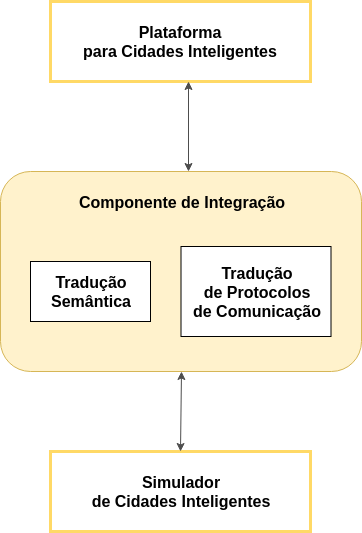
\includegraphics[width=0.4\textwidth]{figuras/integration-general-architecture.png}
	\caption{Arquitetura Proposta para Ambiente Integrado de Exerimentação de Plataformas de Cidades Inteligentes}
	\label{fig:general_architecture}
\end{figure}


Na Figura \ref{fig:general_architecture}, podemos ver os componentes presentes na arquitetura de integração do sistema aqui apresentada.
Como elucidado anteriormente, o componente de integração não pode possuir muitas responsabilidades, já que uma complexidade alta pode acarretar em um aumento expressivo no
tempo de transmissão dos dados, sendo esse um requisito importante para o sistema.
Já as ferramentas envolvidas, além de suas próprias funcionalidades, esperamos que as mesmas possuam um módulo de comunicação para suportar o fluxo de dados em tempo de execução.

O componente de integração tem a responsabilidade de solucionar os pontos mencionados anteriormente:

\begin{itemize}
    \item Tradução semântica entre o simulador e a plataforma

    \item Interoperação entre protocolos de rede

    \item Interferência mínima no tempo de envio e recebimento de dados
\end{itemize}

Como pode ser visto, o componente de integração tem como único objetivo atender requisitos não funcionais.
Ele deve tornar a comunicação do simulador e da plataforma transparente para ambos e adicionando a menor complexidade possível ao sistema.

Em resumo, devemos escolher ferramentas (simulador e plataforma) mais semelhantes possíveis, com o que diz respeito principalmente ao modelo conceitual e aos protocolos de
rede utilizados para comunicação; e implementar o componente de integração o mais simples possível, apenas com o objetivo de viabilizar a comunicação entre as ferramentas.

